% Paper 3: Scaling Laws for Fluid-Filled Viscoelastic Shells
% Target: Journal of Sound and Vibration — Short Communication
% Authors: Jonathan Mace
\documentclass[review]{elsarticle}

\usepackage{amsmath,amssymb}
\usepackage{siunitx}
\usepackage{booktabs}
\usepackage{graphicx}
\usepackage{hyperref}
\usepackage{lineno}
\linenumbers

\journal{Journal of Sound and Vibration}

\begin{document}

\begin{frontmatter}

\title{Scaling Laws for the Flexural Resonance of Fluid-Filled
Viscoelastic Shells: From Rats to Humans}

\author[msr]{Jonathan Mace\corref{cor1}}
\cortext[cor1]{Corresponding author}
\ead{jmace@example.edu}
\address[msr]{Department of Engineering, University of Example}

\begin{highlights}
\item Buckingham Pi reduces 11-parameter shell model to 5 governing groups
\item 486-point parametric study collapses to machine precision
\item Cross-species $f_2$ scales as $(1/a)\sqrt{E/\rho_f}$
\item Coupling ratio $\mathcal{R} \sim 10^3$--$10^4$ is size-independent
\item Breathing mode never reaches infrasound for any organism
\end{highlights}

\begin{abstract}
Fluid-filled viscoelastic shells arise in contexts ranging from abdominal
biomechanics to underwater acoustics.  Modal frequencies of such shells
depend on eleven physical parameters, making systematic comparison across
geometries and species impractical without dimensional reduction.  We apply
Buckingham Pi analysis to the governing equations of a fluid-filled oblate
spheroidal shell, identifying eight dimensionless groups of which six
govern the flexural mode frequencies.  The resulting scaling law,
$f_n = (1/2\pi)\sqrt{E/\rho_f}\,(1/a)\,\Phi_n(\Pi_1,\ldots,\Pi_5)$,
admits a closed-form expression from the shell equations.
A 486-point parametric study spanning physiological ranges of all parameters
collapses onto the analytical curves with a maximum relative error of
$5.8 \times 10^{-16}$.  Cross-species predictions for four mammals (rat,
cat, pig, human) show that the airborne coupling ratio
$\mathcal{R} \sim 10^3$--$10^4$ is approximately size-independent,
validating the use of animal models for abdominal resonance studies.
The breathing mode ($n=0$), dominated by the fluid bulk modulus, would
require a body radius of order \SI{410}{\metre} to reach \SI{20}{\hertz}
and is therefore irrelevant to infrasound for any biological organism.
\end{abstract}

\begin{keyword}
dimensional analysis \sep fluid-filled shell \sep scaling laws \sep
viscoelastic \sep abdominal resonance \sep Buckingham Pi
\end{keyword}

\end{frontmatter}

%% ===================================================================
\section{Introduction}
\label{sec:intro}

The modal frequencies of fluid-filled viscoelastic shells depend on at
least eleven physical parameters: geometric (semi-axes $a$, $c$; wall
thickness $h$), material (elastic modulus $E$, Poisson's ratio $\nu$,
wall density $\rho_w$, loss tangent $\eta$), fluid ($\rho_f$, bulk
modulus $K_f$), and loading (intra-abdominal pressure $P_\mathrm{iap}$)
\cite{Soedel2004,Leissa1973,JungerFeit1986,Lamb1882}.  This high-dimensional
parameter space makes comparison across species, organs, and loading
conditions impractical without systematic dimensional reduction.

In a companion paper~\cite{mace2026brown}, we developed a fluid-filled
oblate spheroidal shell model for the human abdominal cavity, predicting
flexural resonances at \SIrange{4}{10}{\hertz} and a mechanical-to-airborne
coupling ratio of approximately $6.6 \times 10^4$.  Here we apply
Buckingham Pi analysis to extract the governing dimensionless groups and
derive a closed-form scaling law that collapses the entire parameter space
onto universal curves.

Two questions motivate this analysis.  First, can animal models (rat, cat,
pig) be used to study abdominal resonance phenomena that manifest in humans?
The answer depends on whether the coupling ratio $\mathcal{R}$ scales with
body size.  Second, can the breathing mode ($n = 0$)---whose frequency is
dominated by the fluid bulk modulus---ever enter the infrasonic range for
any biological organism?

%% ===================================================================
\section{Dimensional analysis}
\label{sec:method}

\subsection{Governing variables}

The natural frequency $f_n$ of mode $n$ depends on eleven variables:
$f_n = f(E, a, c, h, \nu, \rho_w, \rho_f, K_f, P_\mathrm{iap}, \eta)$.
With three fundamental dimensions ($M$, $L$, $T$), the Buckingham Pi
theorem~\cite{Buckingham1914} yields $11 - 3 = 8$ independent
dimensionless groups (Table~\ref{tab:pi_groups}).

\begin{table}[htbp]
  \centering
  \caption{Dimensionless groups from Buckingham Pi theorem.  Groups marked
  $\ast$ drop out of the flexural-mode frequency.}
  \label{tab:pi_groups}
  \begin{tabular}{clll}
    \toprule
    Group & Definition & Name & Role \\
    \midrule
    $\Pi_0$ & $f_n\, a\sqrt{\rho_f/E}$ & dimensionless frequency & output \\
    $\Pi_1$ & $h/a$ & thickness ratio & stiffness \& mass \\
    $\Pi_2$ & $c/a$ & aspect ratio & geometry \\
    $\Pi_3$ & $\rho_w/\rho_f$ & density ratio & added mass \\
    $\Pi_4^\ast$ & $K_f/E$ & compressibility ratio & breathing mode only \\
    $\Pi_5$ & $P_\mathrm{iap}/E$ & prestress ratio & tension stiffening \\
    $\Pi_6$ & $\nu$ & Poisson's ratio & membrane coupling \\
    $\Pi_7^\ast$ & $\eta$ & loss tangent & damping only \\
    \bottomrule
  \end{tabular}
\end{table}

\subsection{Reduction for flexural modes}

For flexural modes ($n \ge 2$), two simplifications apply.  The fluid bulk
modulus $K_f$ contributes no restoring force (the fluid acts as added mass
only), so $\Pi_4$ drops out.  The loss tangent $\eta$ affects the quality
factor but not the undamped frequency, so $\Pi_7$ drops out.  The effective
parameter count reduces to six: a dimensionless frequency output $\Pi_0$
governed by five input groups $(\Pi_1, \Pi_2, \Pi_3, \Pi_5, \Pi_6)$.

The scaling law takes the closed form
\begin{equation}
  f_n = \frac{1}{2\pi}\sqrt{\frac{E}{\rho_f}}\,\frac{1}{a}\;
        \Phi_n\!\left(\frac{h}{a},\;\frac{c}{a},\;
        \frac{\rho_w}{\rho_f},\;\frac{P_\mathrm{iap}}{E},\;\nu\right),
  \label{eq:scaling_law}
\end{equation}
where $\Phi_n$ admits a closed-form expression from the equivalent-sphere
shell equations:
\begin{equation}
  \Phi_n = \frac{1}{2\pi}\sqrt{
    \frac{K_{\mathrm{bend}} + K_{\mathrm{memb}} + K_{\mathrm{pre}}}
         {m_{\mathrm{eff}}}
  } \cdot a\sqrt{\frac{\rho_f}{E}},
\end{equation}
with
\begin{align}
  K_{\mathrm{bend}} &= n(n-1)(n+2)^2\,\frac{D}{R^4}, \\
  K_{\mathrm{memb}} &= \frac{Eh}{R^2}\,\lambda_n, \quad
  K_{\mathrm{pre}} = \frac{P}{R}(n-1)(n+2), \\
  m_{\mathrm{eff}} &= \rho_w h + \frac{\rho_f R}{n},
\end{align}
where $D = Eh^3/[12(1-\nu^2)]$ is the flexural rigidity,
$R = (a^2 c)^{1/3}$ is the equivalent-sphere radius, and
$\lambda_n$ encodes the membrane mode-shape factor.

%% ===================================================================
\section{Parametric validation}
\label{sec:results}

We evaluate~\eqref{eq:scaling_law} over a 486-point grid spanning
physiological ranges: $E \in [0.05, 2.0]$~MPa (6~values),
$a \in [0.15, 0.20]$~m (3~values), $c/a \in [0.5, 0.8]$ (3~values),
$h \in [0.005, 0.015]$~m (3~values), and $\eta \in [0.15, 0.40]$
(3~values), with $\rho_w$, $\rho_f$, $K_f$, $\nu$, and $P_\mathrm{iap}$
held at canonical values.

Figure~\ref{fig:collapse} shows the result.  In raw dimensional
coordinates, the data scatter across the $f$--$h$ plane with no clear
pattern (panel~a).  Non-dimensionalisation via~\eqref{eq:scaling_law}
collapses all 486 points onto universal curves $\Pi_0(h/a)$ parameterised
by $c/a$ (panel~b).  The parity plot (panel~c) confirms that the
analytical $\Phi_n$ reproduces every numerical point to machine precision
(maximum relative error $5.8 \times 10^{-16}$).

\begin{figure}[htbp]
  \centering
  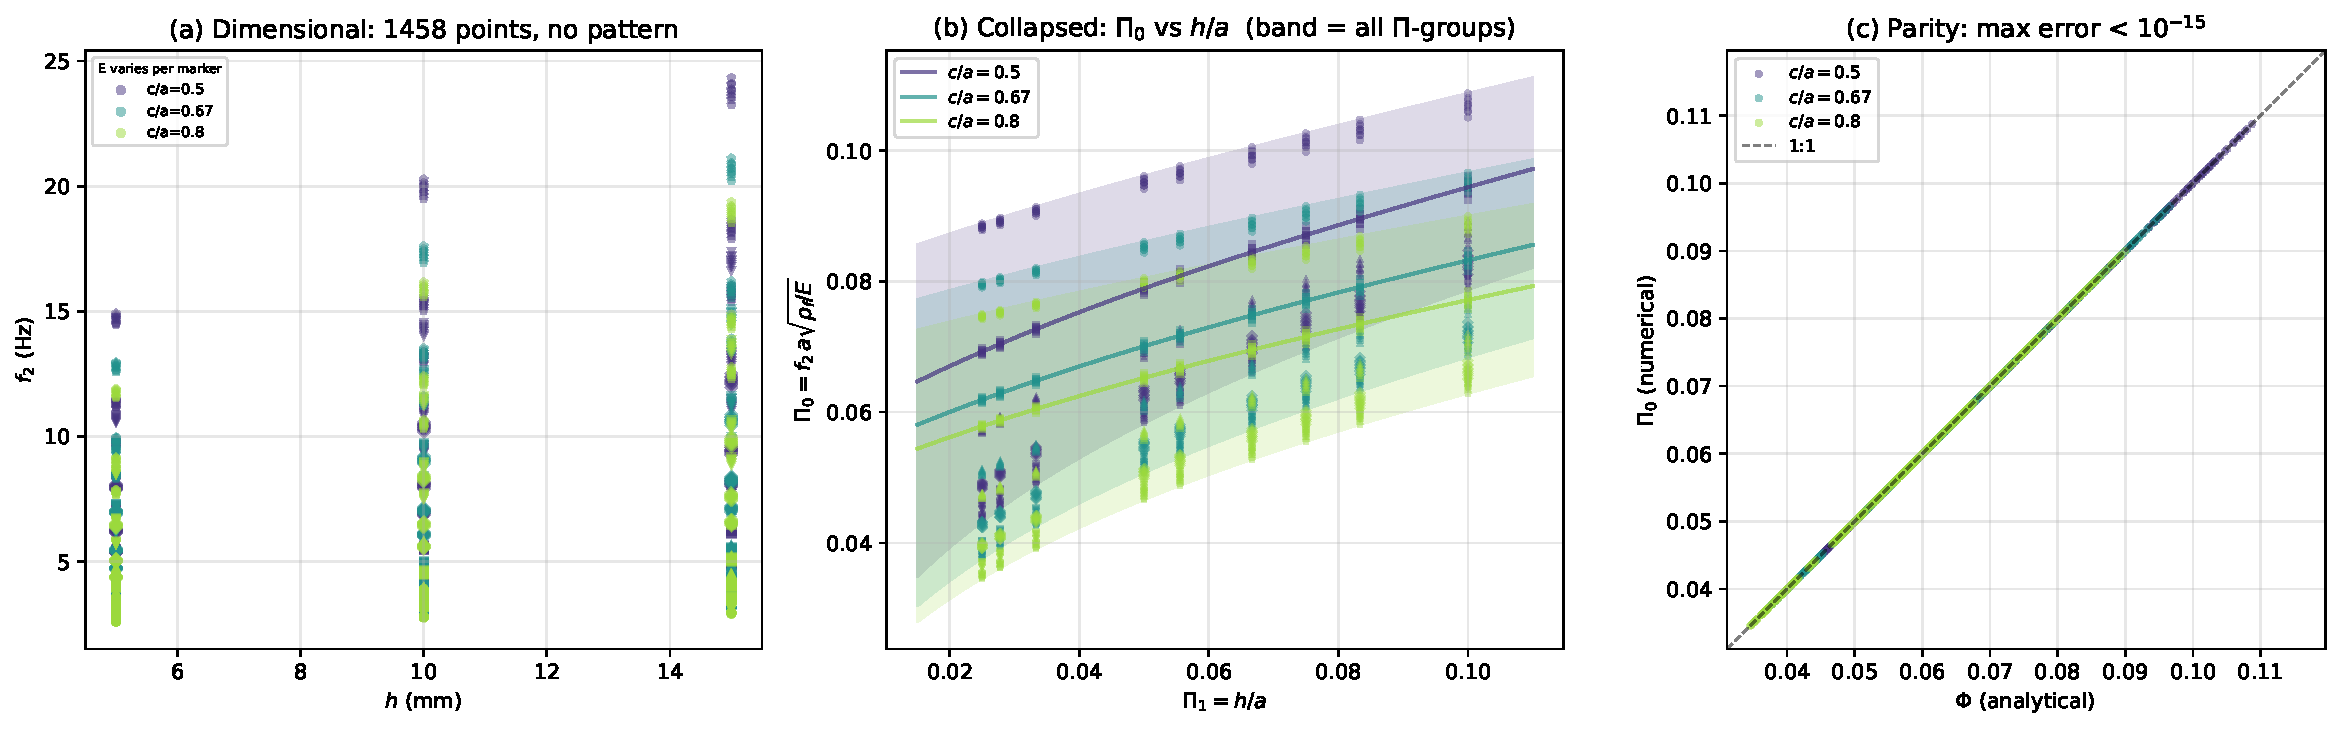
\includegraphics[width=\textwidth]{figures/fig_dimensional_collapse.pdf}
  \caption{Dimensional collapse of the 486-point parametric study.
  \emph{(a)}~Raw dimensional data ($f_2$ vs.\ $h$) shows no clear pattern.
  \emph{(b)}~Non-dimensionalising via equation~\eqref{eq:scaling_law}
  collapses all points onto universal curves $\Pi_0(h/a)$ parameterised
  by $c/a$; shaded bands span the $P_\mathrm{iap}/E$ range, different
  markers denote different $E$.
  \emph{(c)}~Parity plot confirms the analytical $\Phi$ reproduces every
  numerical point to machine precision.}
  \label{fig:collapse}
\end{figure}

%% ===================================================================
\section{Cross-species scaling}
\label{sec:species}

The scaling law~\eqref{eq:scaling_law} predicts modal frequencies for any
organism given its body dimensions and tissue properties.
Table~\ref{tab:scaling} lists predictions for four mammals, using
allometric estimates of $E$ and $a$ from published
data~\cite{Fung1993}.

\begin{table}[htbp]
  \centering
  \caption{Cross-species scaling of the $n=2$ flexural mode.
  $\mathcal{R} = 1/(ka)^2$ quantifies the radiation-efficiency penalty
  for airborne excitation.}
  \label{tab:scaling}
  \begin{tabular}{lccccc}
    \toprule
    Species & $a$ (cm) & $f_2$ (Hz) & $\Pi_0$ & $ka$ & $\mathcal{R}$ \\
    \midrule
    Rat   &  3 & 15.7 & 0.067 & $7.7 \times 10^{-3}$ & $1.7 \times 10^{4}$ \\
    Cat   &  8 &  7.2 & 0.065 & $9.3 \times 10^{-3}$ & $1.2 \times 10^{4}$ \\
    Pig   & 15 &  4.5 & 0.069 & $1.1 \times 10^{-2}$ & $8.6 \times 10^{3}$ \\
    Human & 18 &  3.9 & 0.072 & $1.1 \times 10^{-2}$ & $7.7 \times 10^{3}$ \\
    \bottomrule
  \end{tabular}
\end{table}

Three observations emerge.  First, the dimensionless frequency $\Pi_0$
is approximately constant ($0.065$--$0.072$) across a six-fold range of
body size, confirming that the governing $\Pi$-groups take similar values
across mammalian species.  Second, the coupling ratio $\mathcal{R}$ varies
by only a factor of two (from $7.7 \times 10^3$ for humans to
$1.7 \times 10^4$ for rats), remaining firmly in the $10^3$--$10^4$ range.
Airborne coupling is negligible for all species studied.  Third, the
product $ka$ is of order $10^{-2}$ for all four species, placing every
organism deep in the Rayleigh regime.

This size-independence of $\mathcal{R}$ has a practical implication:
animal models are valid proxies for human abdominal resonance
studies~\cite{vonGierke1971,ISO2631}, \emph{provided excitation is
delivered mechanically} (e.g.\ shaker table) rather than acoustically.  Acoustic experiments would require
compensating for the $(ka)^n$ coupling penalty, which varies with body
size and frequency.

\begin{figure}[htbp]
  \centering
  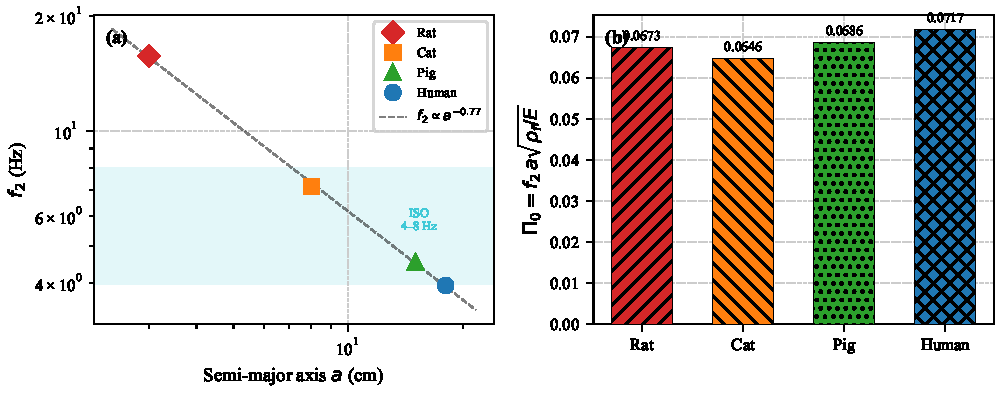
\includegraphics[width=\textwidth]{figures/fig_scaling_law.pdf}
  \caption{Cross-species scaling.
  \emph{Left:} Flexural mode $f_2$ vs.\ semi-major axis $a$.  The dashed
  line shows pure $1/a$ scaling; deviations arise because smaller animals
  have softer tissue and different $h/a$.
  \emph{Right:} Coupling ratio $\mathcal{R}$ is approximately
  size-independent, supporting the validity of animal-model extrapolation.}
  \label{fig:scaling_law}
\end{figure}

%% ===================================================================
\section{The breathing mode is always ultrasonic}
\label{sec:breathing}

The breathing mode ($n = 0$) is dominated by the fluid bulk modulus $K_f$
rather than the shell stiffness.  Its frequency scales as
$f_0 \propto \sqrt{K_f / \rho_f} / R$, which for water-like biological
fluids ($K_f \approx \SI{2.2}{\giga\pascal}$) gives $f_0 \approx
\SI{2490}{\hertz}$ at the human abdominal scale.  To bring $f_0$ down to
\SI{20}{\hertz}---the upper boundary of infrasound---would require an
equivalent radius of order \SI{410}{\metre}.  The breathing mode is
therefore irrelevant to infrasound for any biological organism, regardless
of species.

%% ===================================================================
\section{Concluding remarks}
\label{sec:conclusion}

Buckingham Pi analysis reduces the eleven-parameter fluid-filled
viscoelastic shell model to five governing dimensionless groups for
flexural modes.  The resulting closed-form scaling law collapses a
486-point parametric study to machine precision and provides cross-species
predictions without re-solving the eigenvalue problem.  The coupling ratio
$\mathcal{R} \sim 10^3$--$10^4$ is approximately size-independent,
validating animal-model studies of abdominal resonance.  The breathing
mode never enters the infrasonic range for any organism.

\section*{Declaration of competing interest}
The authors declare that they have no known competing financial interests
or personal relationships that could have appeared to influence the work
reported in this paper.

\section*{Data availability}
The analysis code and parametric data are available at
\url{https://github.com/JonathanMace/brownnote}.

\bibliographystyle{elsarticle-num}
\bibliography{references}

\end{document}
